\documentclass[border=4pt]{standalone}

\usepackage{tikz}

\definecolor{otblue}{HTML}{0072B2}
\definecolor{otorange}{HTML}{E69F00}
\definecolor{otteal}{HTML}{009E73}
\definecolor{otpurple}{HTML}{CC79A7}
\definecolor{otgray}{HTML}{5A5A5A}

\begin{document}
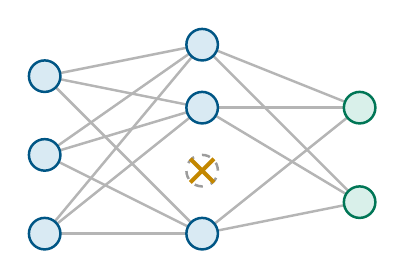
\begin{tikzpicture}[line width=0.9pt]
  \foreach \y in {0,1,2}{\foreach \t in {0,1.6,2.4}{\draw[otgray!45] (0,\y) -- (2,\t);}}
  \foreach \t in {0,1.6,2.4}{\foreach \z in {0.4,1.6}{\draw[otgray!45] (2,\t) -- (4,\z);}}
  \foreach \y in {0,1,2}{\filldraw[draw=otblue!75!black, fill=otblue!15] (0,\y) circle[radius=0.2];}
  \foreach \t in {0,1.6,2.4}{\filldraw[draw=otblue!75!black, fill=otblue!15] (2,\t) circle[radius=0.2];}
  \filldraw[draw=otgray!60, fill=white, dashed] (2,0.8) circle[radius=0.2];
  \draw[otorange!85!black, line width=1.5pt] (1.85,0.65) -- (2.15,0.95) (1.85,0.95) -- (2.15,0.65);
  \foreach \y in {0.4,1.6}{\filldraw[draw=otteal!75!black, fill=otteal!15] (4,\y) circle[radius=0.2];}
\end{tikzpicture}
\end{document}
